\chapter{总结}
\label{cha:Conclusion}

本文提出了一种用于智能电网分布式算法开发测试的集群交互平台,同时也是一个全新的桌面级实物集群交互开发平台,如图~\ref{fig:model}。

\begin{figure}[htbp]
    \centering
    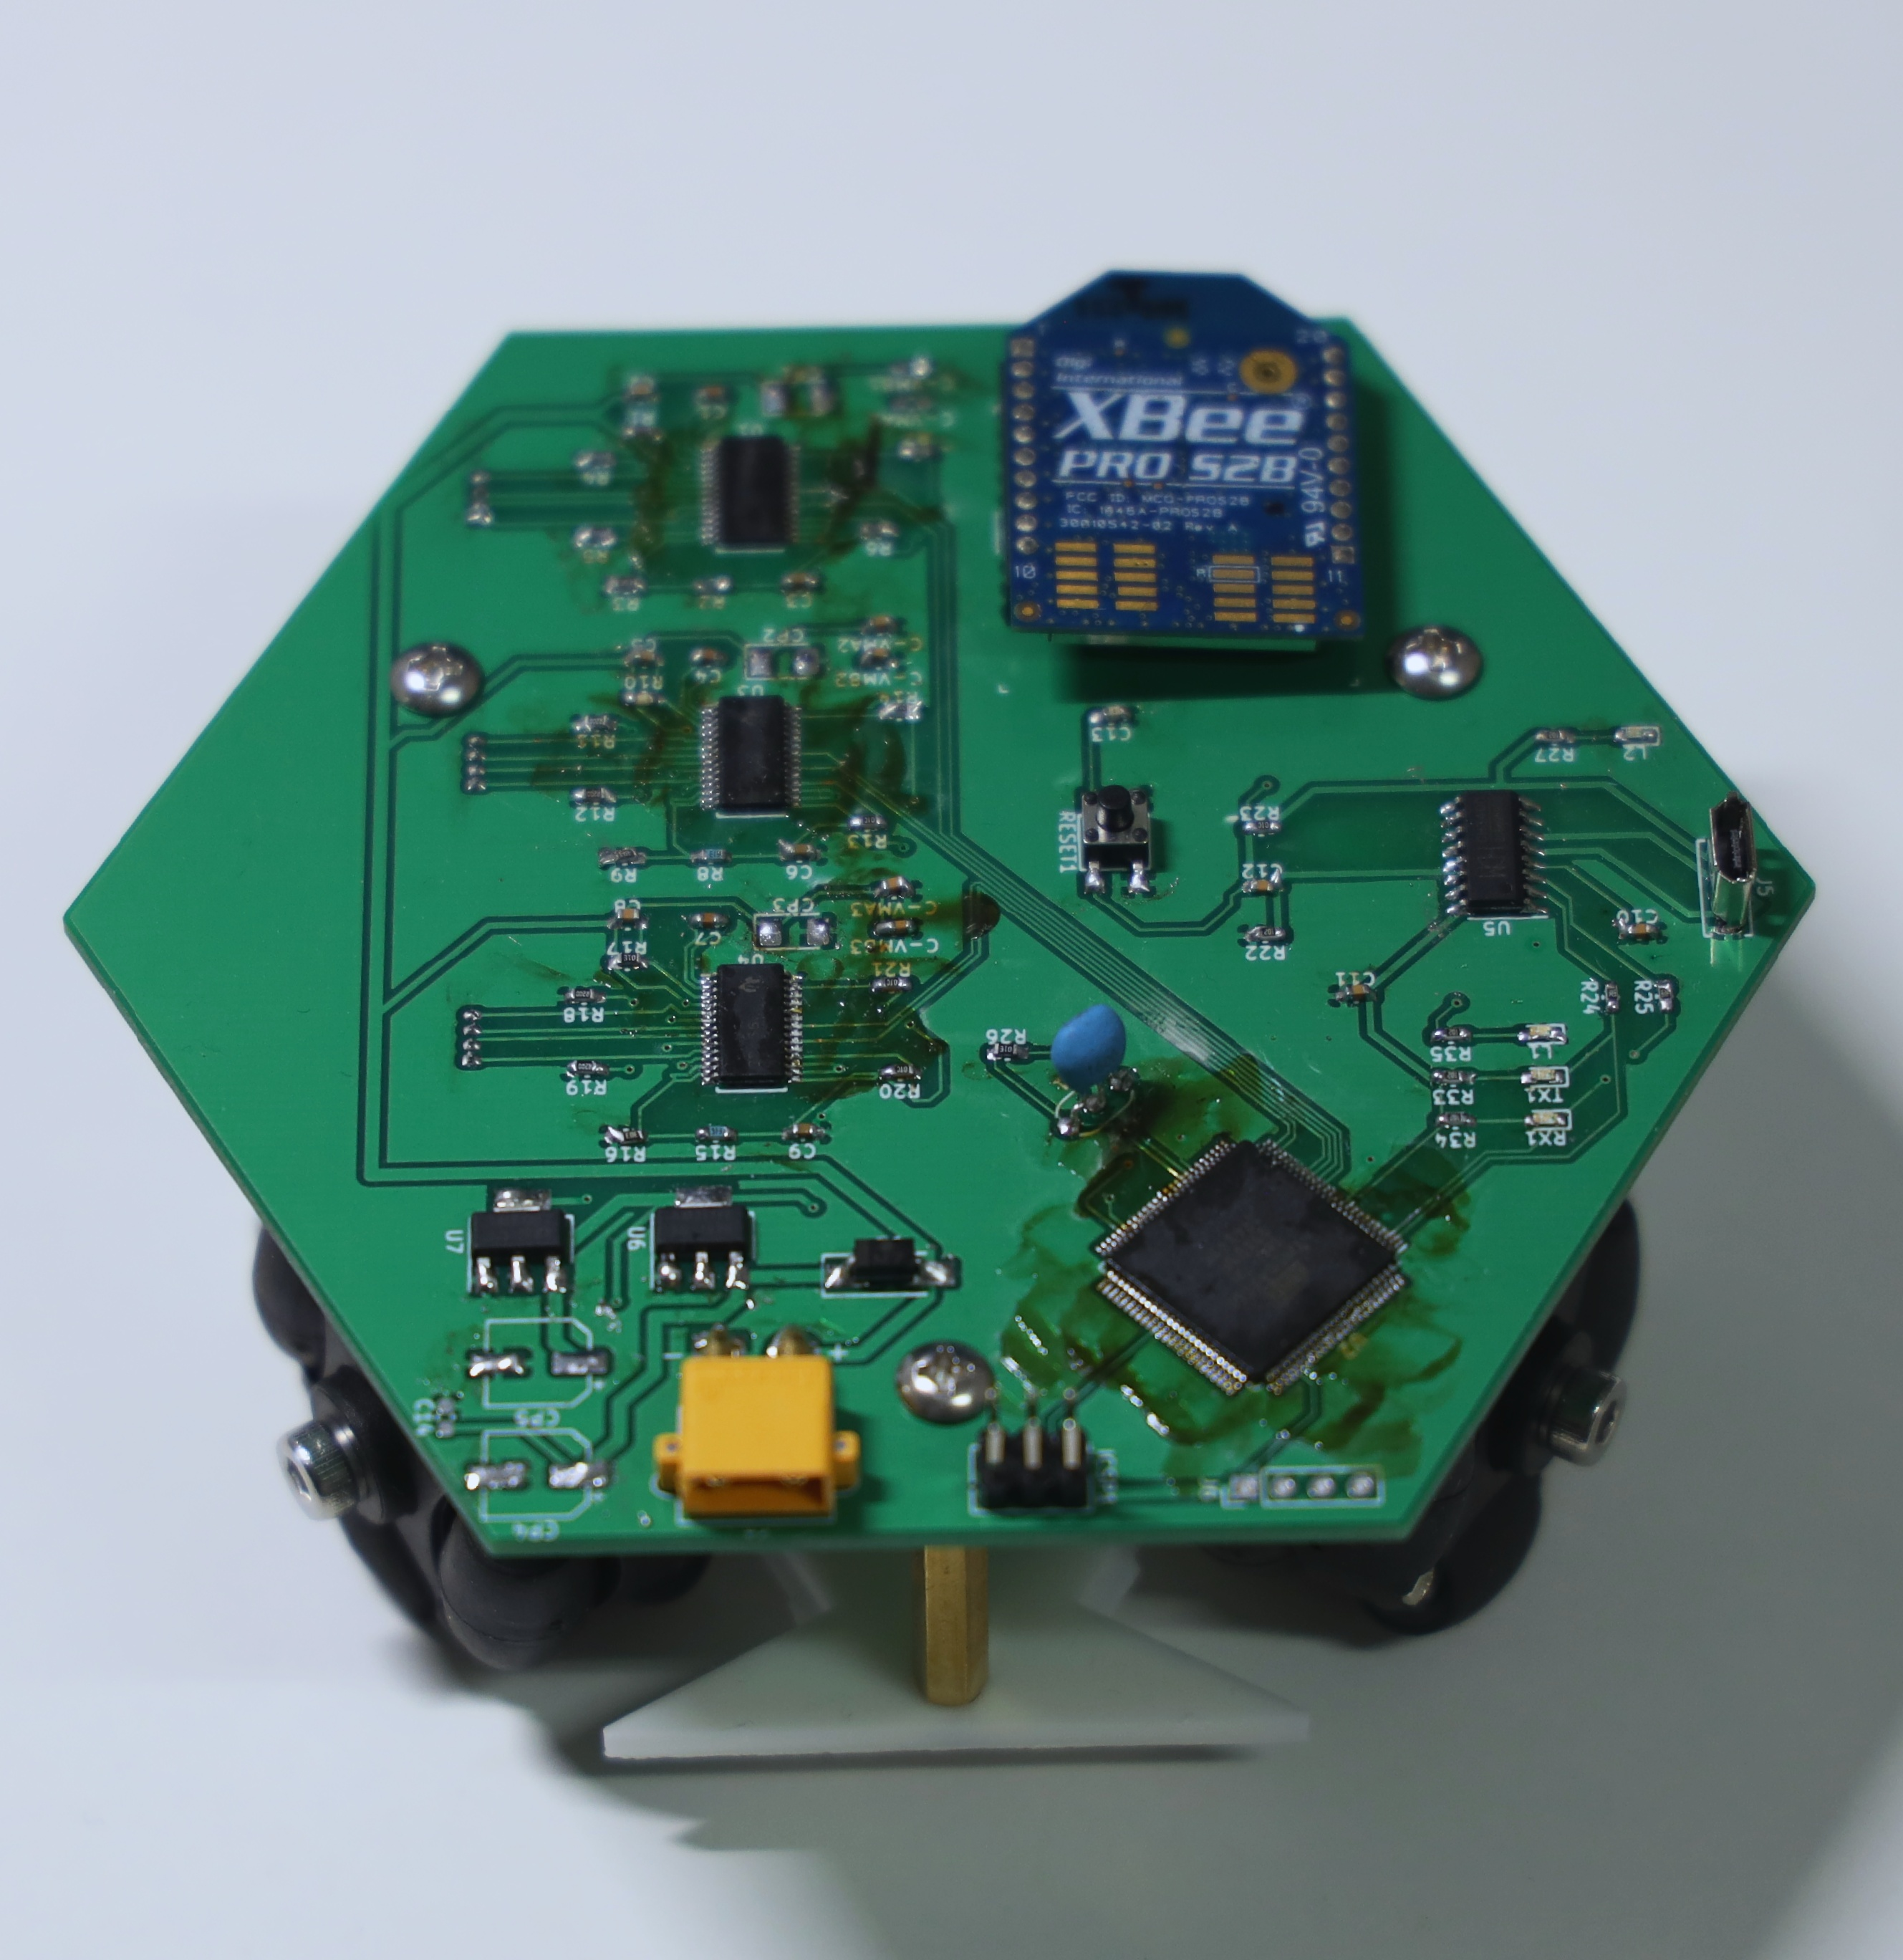
\includegraphics[width=0.8\columnwidth]{model.jpg}
    \caption{平台单元}
    \label{fig:model}
\end{figure}

同时提出了一种简化的完全去中心化的平均值共识算法,以解决未来智能电网中的经济调度问题,并以各种方式使用交互平台对其可视化,如图~\ref{fig:iteration}。

\begin{figure}[htbp]
    \centering
    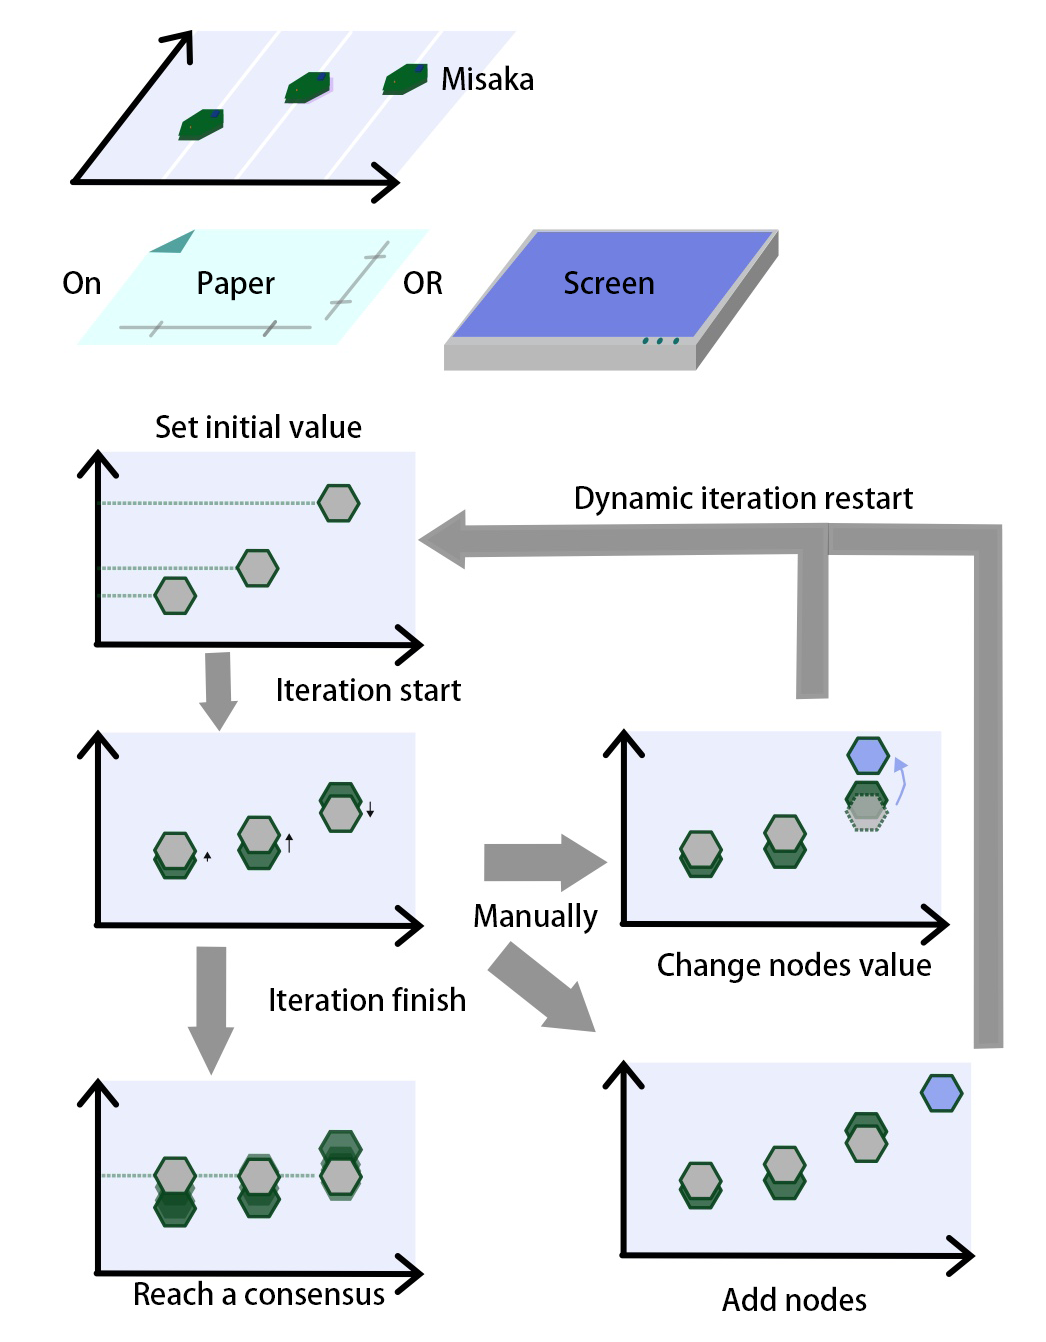
\includegraphics[width=\columnwidth]{Iteration.png}
    \caption{动态迭代可视化}
    \label{fig:iteration}
\end{figure}

希望本文提出的这一平台能够激发更多关于智能电网分布式算法的开发和实物人机交互方式的研究。为了将来的进一步研究工作,开发过程中预留了UART/I2C等接口,目前平台兼容的扩展功能就有人工智能平台/Wifi/BLE等等,如图~\ref{fig:extension}。

\begin{figure}[htbp]
    \centering
    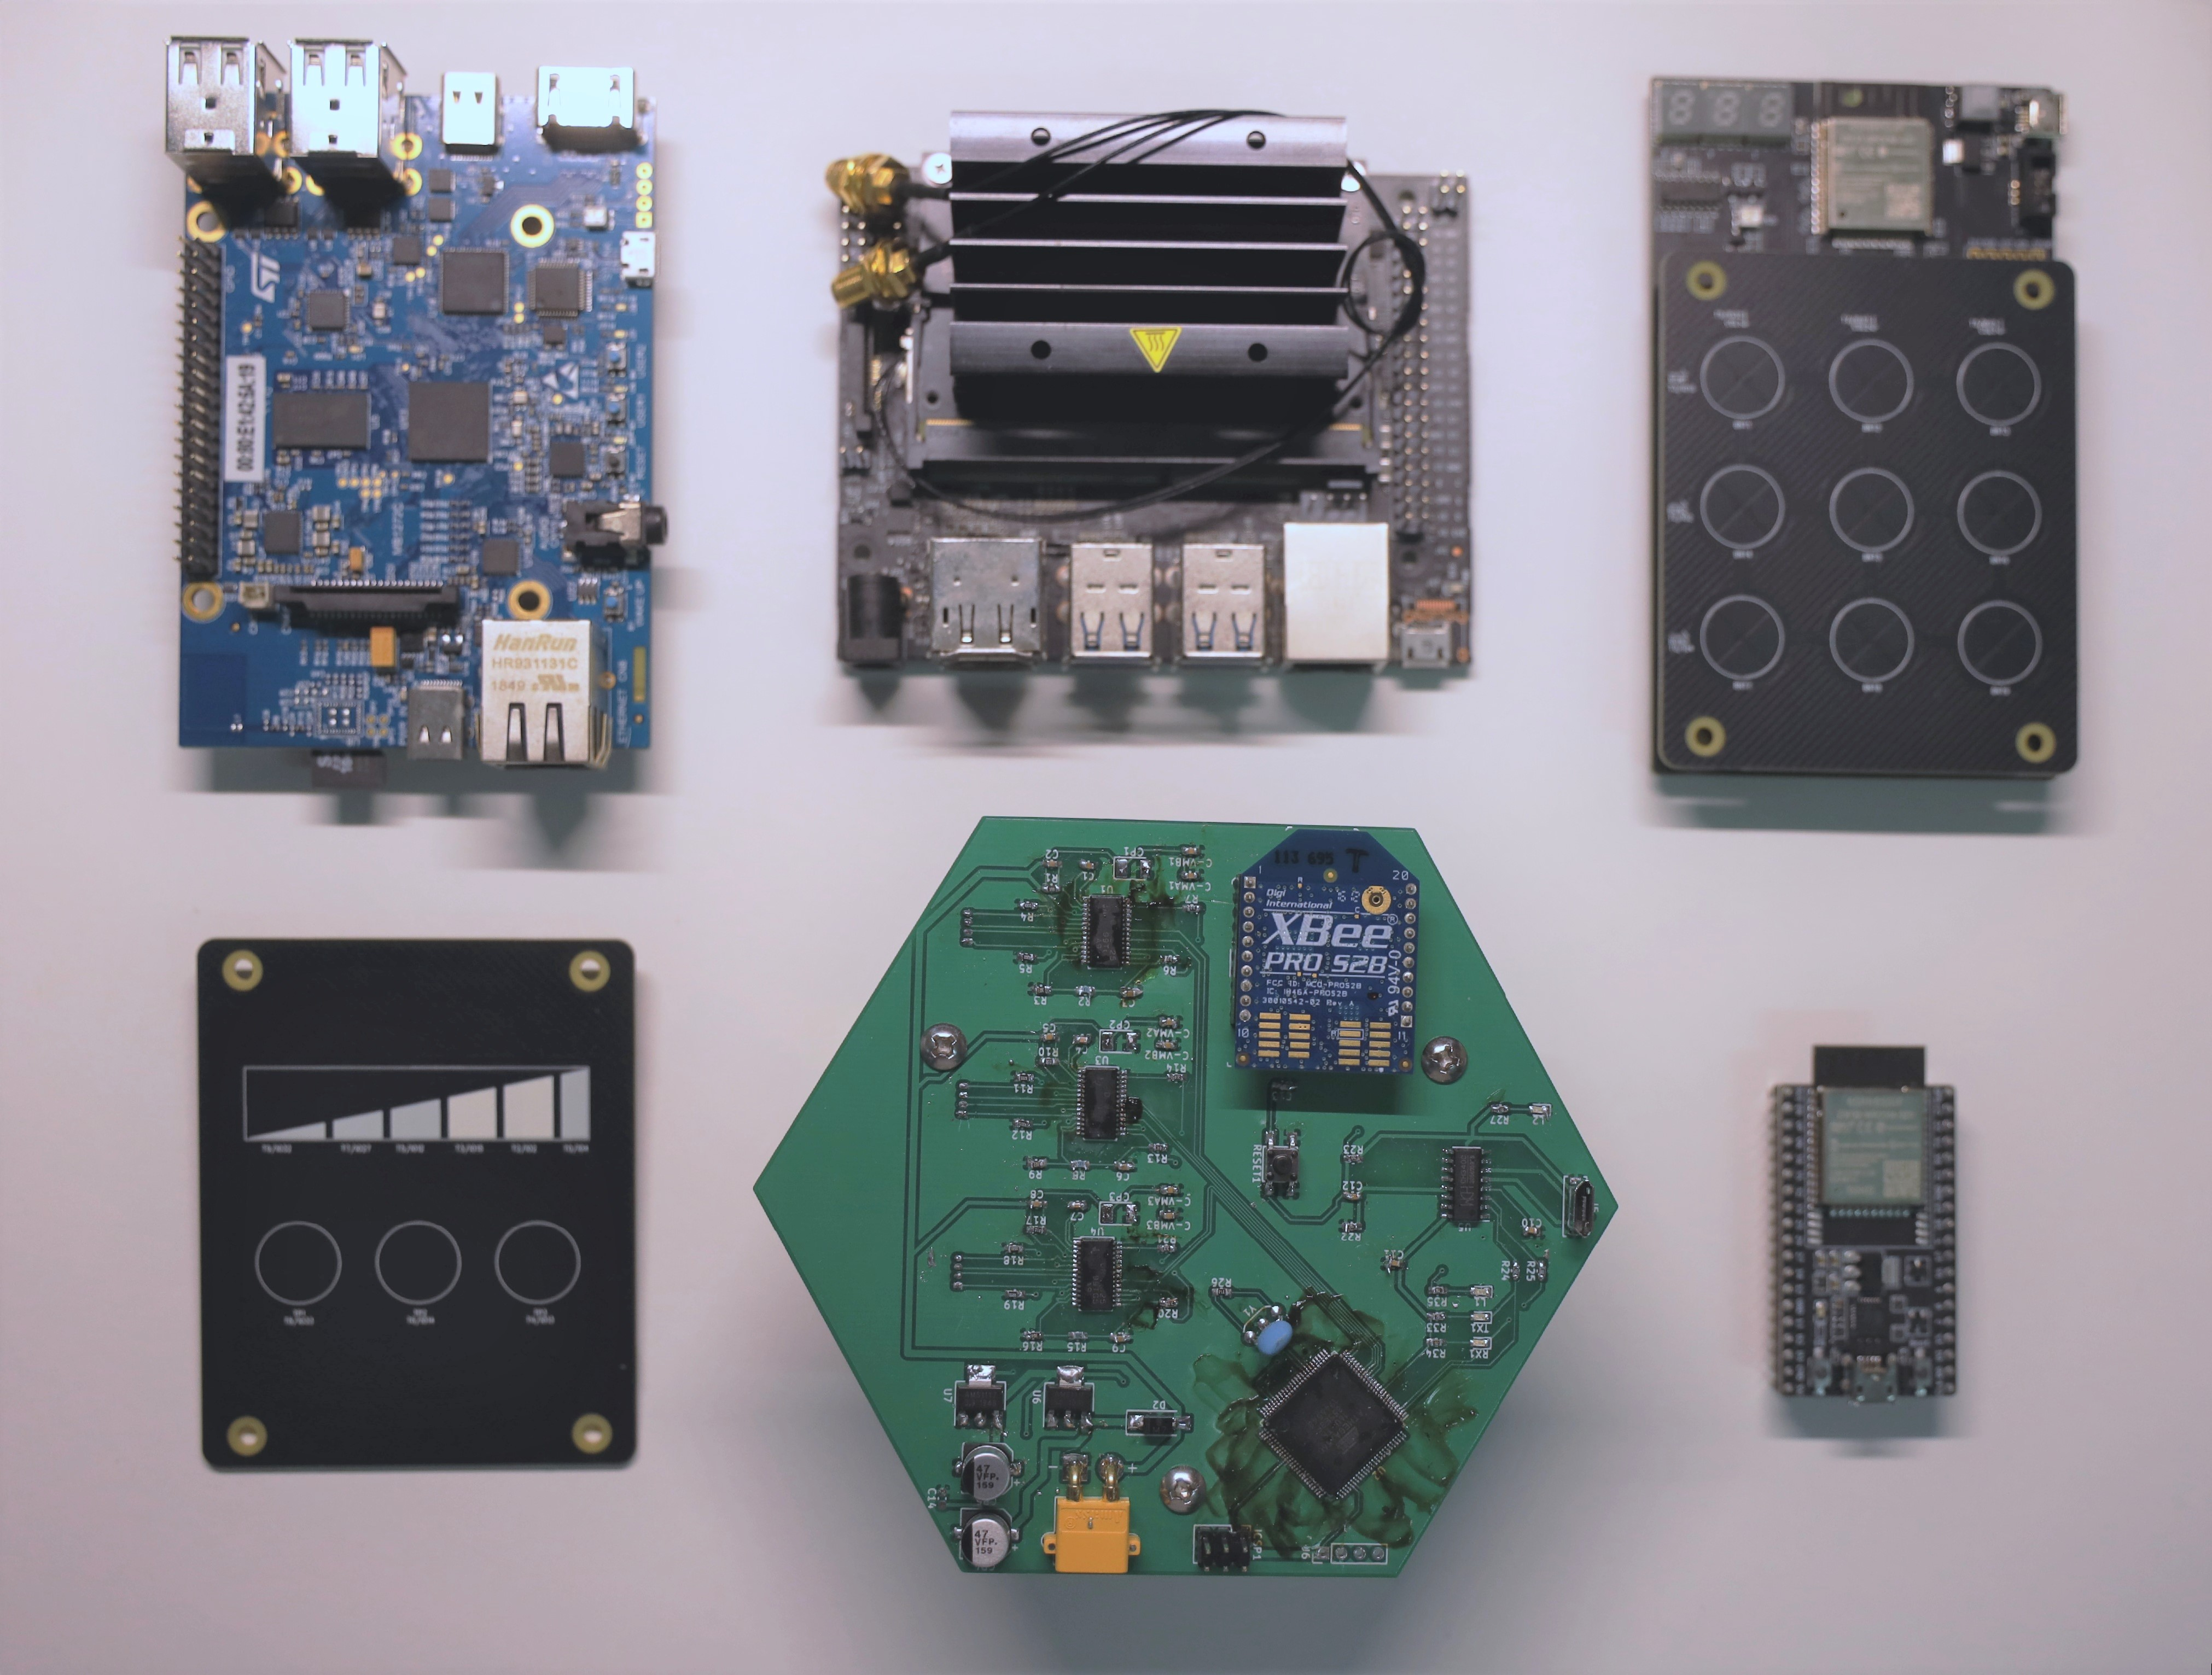
\includegraphics[width=\columnwidth]{extensions.jpg}
    \caption{平台核心和支持的扩展模块}
    \label{fig:extension}
\end{figure}

本平台的所有软硬件资料均在Github上完全开源,包括PCB设计源文件、UI源码、3D打印模型、嵌入式代码、开发笔记和使用说明等:

\url{https://github.com/TingliangZhang/Misaka}

DEMO视频见下:

\url{https://www.bilibili.com/video/BV1Zz4y1R76r/}